%!TEX root = ../document.tex
\chapter{基于双向长短期记忆网络的序列感知推荐算法}

推荐系统面临的问题主要有两大类:评分预测和项目推荐。所以在推荐领域根据用户的历史活动记录预测%
用户下一次行为可能会选择什么项目也是一个重要的问题。在许多在线网站和应用程序当中,如在线电子%
商务、新闻或视频推荐网站、音乐或广播电台,它们都需要为用户提供一个杰出服务来推荐用户在未来可能%
会喜欢的东西。现有的推荐系统主要关注于找出用户或项目的近邻集,或者利用隐式或显式信息(如标签、%
评论、物品内容、用户属性)来提升近邻感知能力。然而,却少有工作利用数据当中的时序属性来直接构建推荐系统。%
在本篇论文中,我们发现数据的序列中其实包含着许多有价值的且激动人心的信息,以视频网站为例,一个用户看%
了纪录片《河西走廊》第一集《使者》之后,接下来看的另一个节目很有可能会是《河西走廊》第二集《通道》。甚至早在%
2011年举办的Recsys推荐系统大会上,来自音乐应用Pandora\footnote{\url{www.pandora.com}}的研究%
人员给出的演讲上都提到了许多用户听音乐具有时序特点。%

在某些特别的应用场景下,常规的推荐系统甚至无法起作用。现有的推荐系统都需要分析用户的数据,因此每个%
网站和应用的使用到需要让用户完成注册以及登录,然而用户每次使用网站或者应用的服务时都不一定会愿意%
登录,这种场景下对匿名用户的推荐显然挑战更大,常规的推荐策略显然无法起作用,基于匿名用户本地浏览器%
和缓存的会话所蕴含的序列进行推荐则显现出很重要的实践意义与价值。

\section{算法框架描述}

为了挖掘许多现有算法忽视掉的用户行为序列特征,本文提出了使用神经网络来对用户的序列进行建模的思路。%
我们的模型(\textit{BiLSTM4Rec})主要由五个部分组成,分别依次是嵌入层、循环结构、全连接层、池化层和输出预测层。其整体框架%
结构如图\ref{fig:structer}所示。

\begin{figure}[htb]
  \centering
  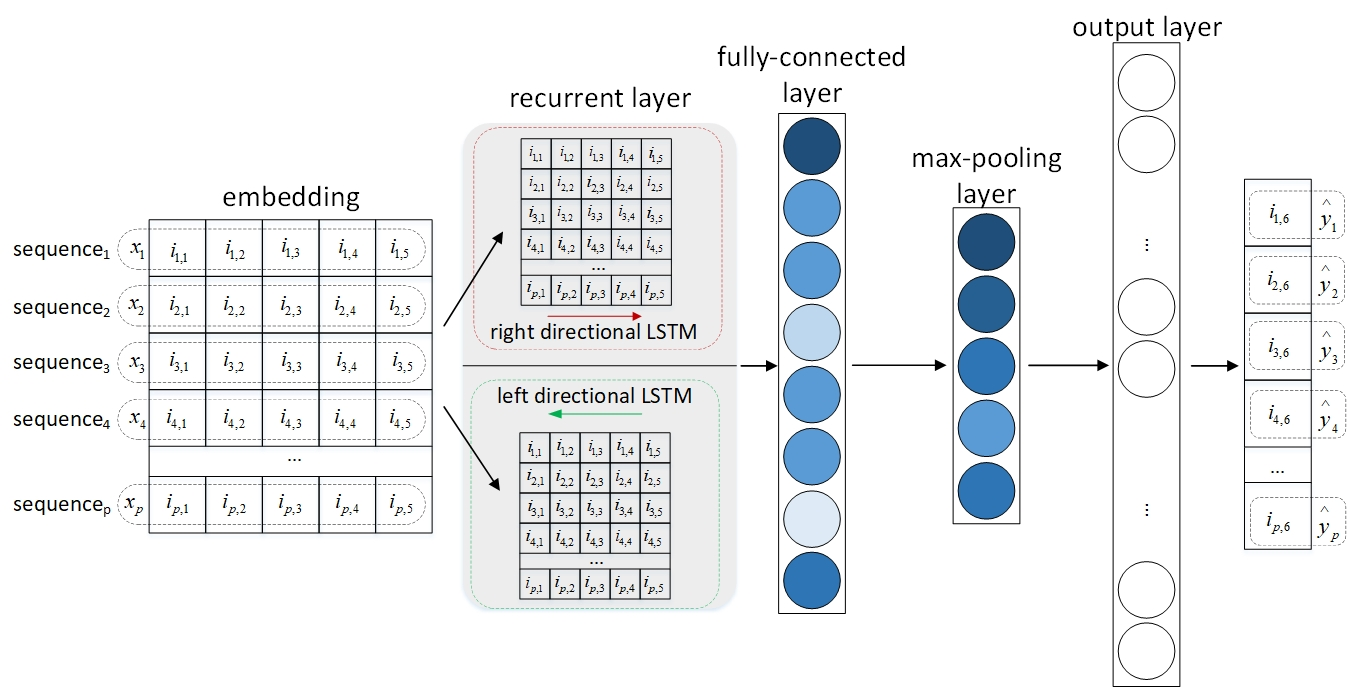
\includegraphics[width=\linewidth]{structer.jpg}\\
  \caption{基于双向循环神经网络的序列推荐算法BiLSTM4Rec框架图}
  \label{fig:structer}
\end{figure}

% \section{基于双向长短期记忆网络的序列感知推荐模型}
\subsection{目标问题定义}

序列感知推荐与传统的单类协同过滤推荐是有很大不同的,序列感知推荐的主要目标是预测用户下一步将会%
点击什么,而且利用数据仅仅包含用户当前历史行为的序列集合,而不接触为用户设置的长期偏好属性。%
接下来我们将定义序列感知这一问题的形式。%

在序列感知推荐当中,我们定义$\mathbb{U}= \left \{ u_{1},u_{2},...,u_{N} \right \}\label{eq}$%
代表不同的用户集合,定义$\mathbb{I}= \left \{ i_{1},i_{2},...,i_{M} \right \}$代表在所有序列%
中出现过的不同物品集合,$s_{u}^{t}\in \mathbb{I}$表示用户$u$在时间刻$t$点击某一个物品的记录,%
该记录对应的物品包含在物品集合$\mathbb{I}$当中。对于每一个用户$u$,%
都记录一个按照数据诞生时间戳顺序排列的用户点击记录%
序列$\mathbb{S}_{u}=\left \{ s_{u}^{1},s_{u}^{2},...,s_{u}^{t-1},s_{u}^{t} \right \}$%
序列感知推荐的目标是预测下一次点击行为,也就是做出$t+1$时刻的推荐$s_{u}^{t+1}$。在序列感知推荐%
模型当中,对于序列$s$,模型的输出是所有候选物品对象可能被点击的概率$\hat{y}$,而概率最大的$K$个%
输出所对应的候选物品将作为推荐项目给到用户。%
%
%
%
%

\subsection{嵌入层}

我们使用用户消费历史的最近几个序列当做特征,用户消费的最后一个物品当做标签,来构建一个超多分类%
的有监督学习模型。因此,在特征工程阶段,我们需要将原始序列特征数据转换为计算机容易处理的向量形式%
并且与标签映射。One\_hot编码是用来表达离散特征的最常用的向量表达形式,然而One\_hot编码的向量会遇%
到高维和稀疏的问题。如果我们使用One\_hot编码来处理具有1000个类别的特征,那么每个特征会被一个拥%
有1000个数字的向量来表示,但其中999个数字会是0。在一个大规模数据集中,就计算效率而言这种方式是%
不可取的。

例如对序列$s_{1},s_{2},s_{3},s_{4},s_{1}$进行One\_hot编码的话,将会得到如图%
\ref{fig:one_hot}的形式
\begin{figure}[htb]
  \centering
  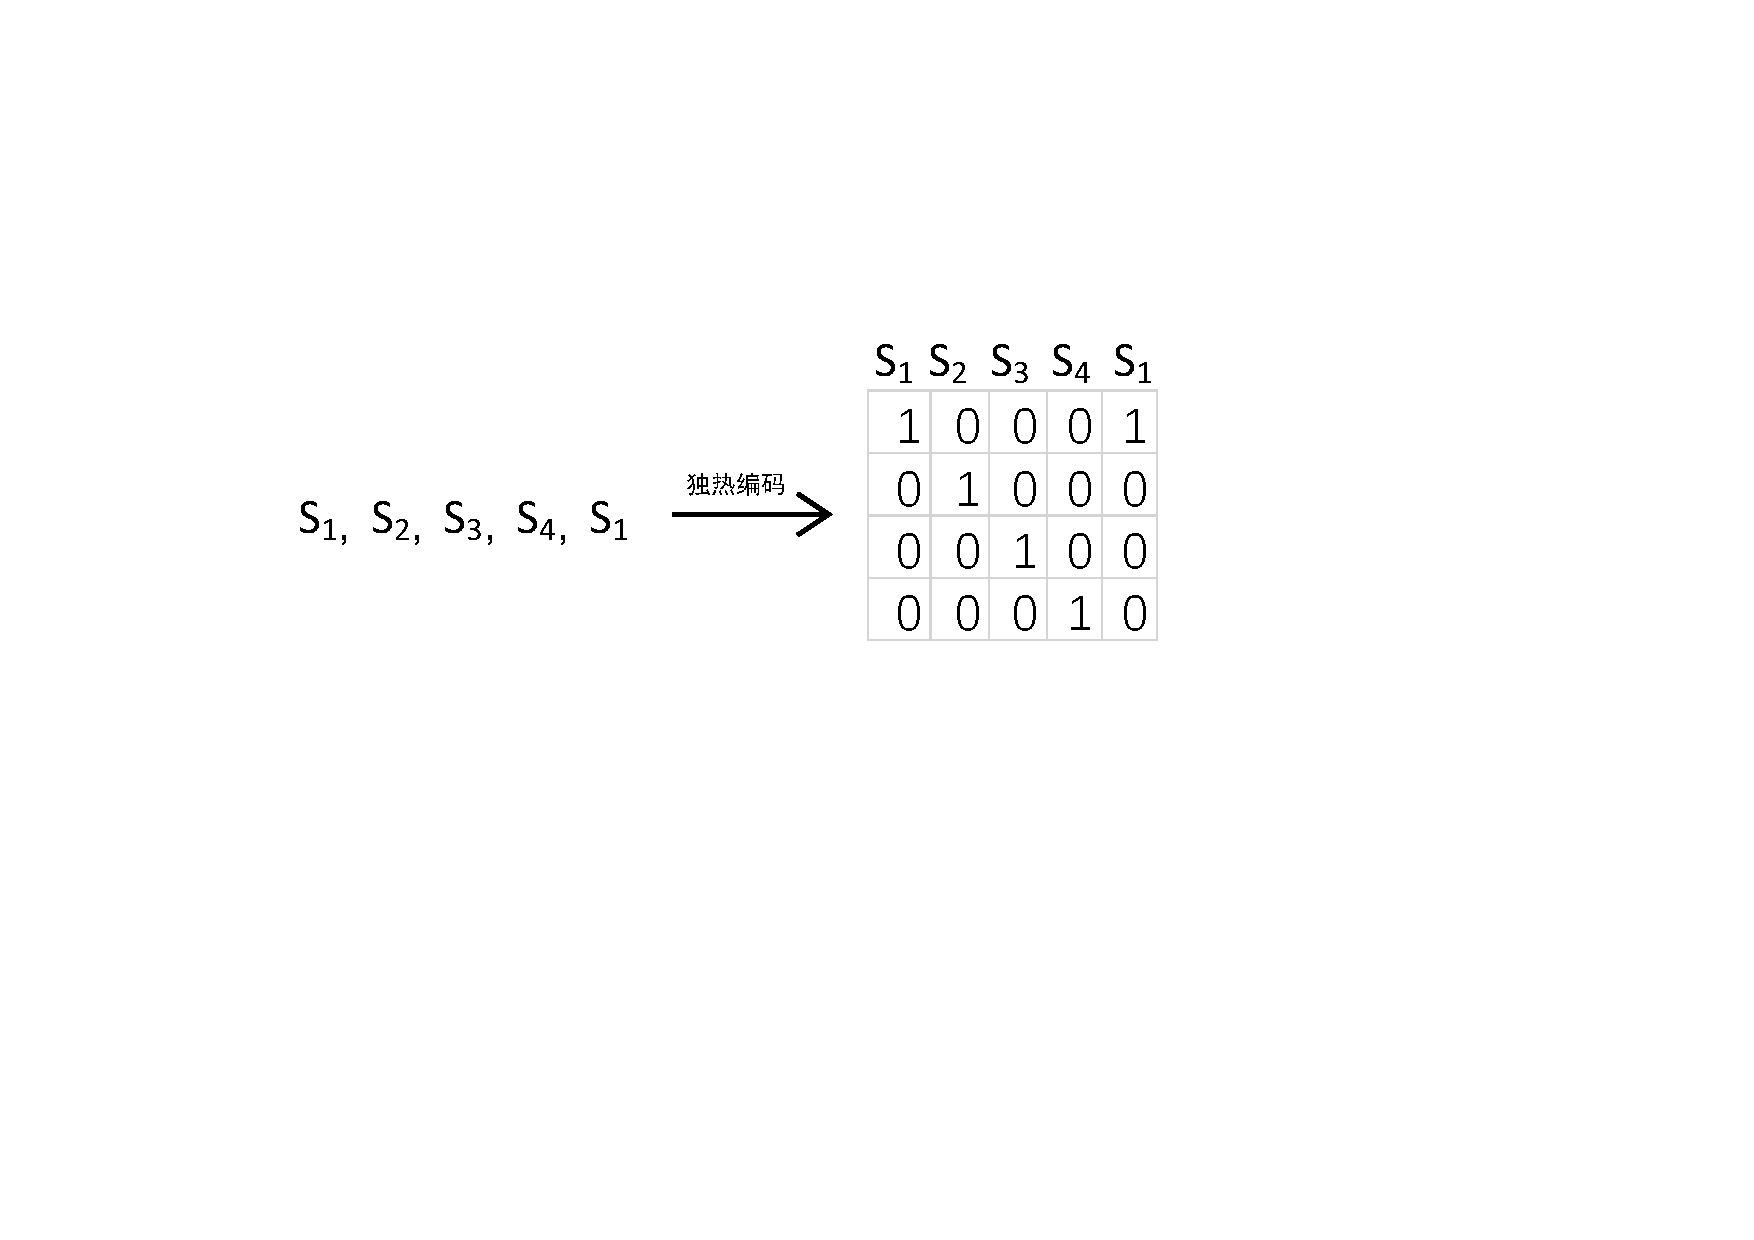
\includegraphics[width=0.6\linewidth]{one_hot.pdf}\\
  \caption{序列独热编码示意图}
  \label{fig:one_hot}
\end{figure}
而词嵌入技术在自然语言处理领域大放异彩,我们可以借用词嵌入技术\upcite{Mikolov:2013:DRW:2999792.2999959},也构造一个嵌入矩阵来%
得到比One\_hot形式小得多的向量结构:
\begin{align}
e(I_i) = EI_i
\end{align}
其中$E\in \mathbb{R}^{|e|\times |M|}$, $|e|$是嵌入层的大小,$|M|$是训练集中不同项目的数量。%
所以$e(I_i)$是$I_i$的嵌入表达,其是一个具有$e$个实数的稠密矩阵。与一个 $|M|\times |M|$大小的%
One\_hot编码形式相比,我们的序列嵌入矩阵的大小为$|e|\times |M|$,当处理大数据集时,这显著减小%
了内存消耗。
\begin{figure}[htb]
  \centering
  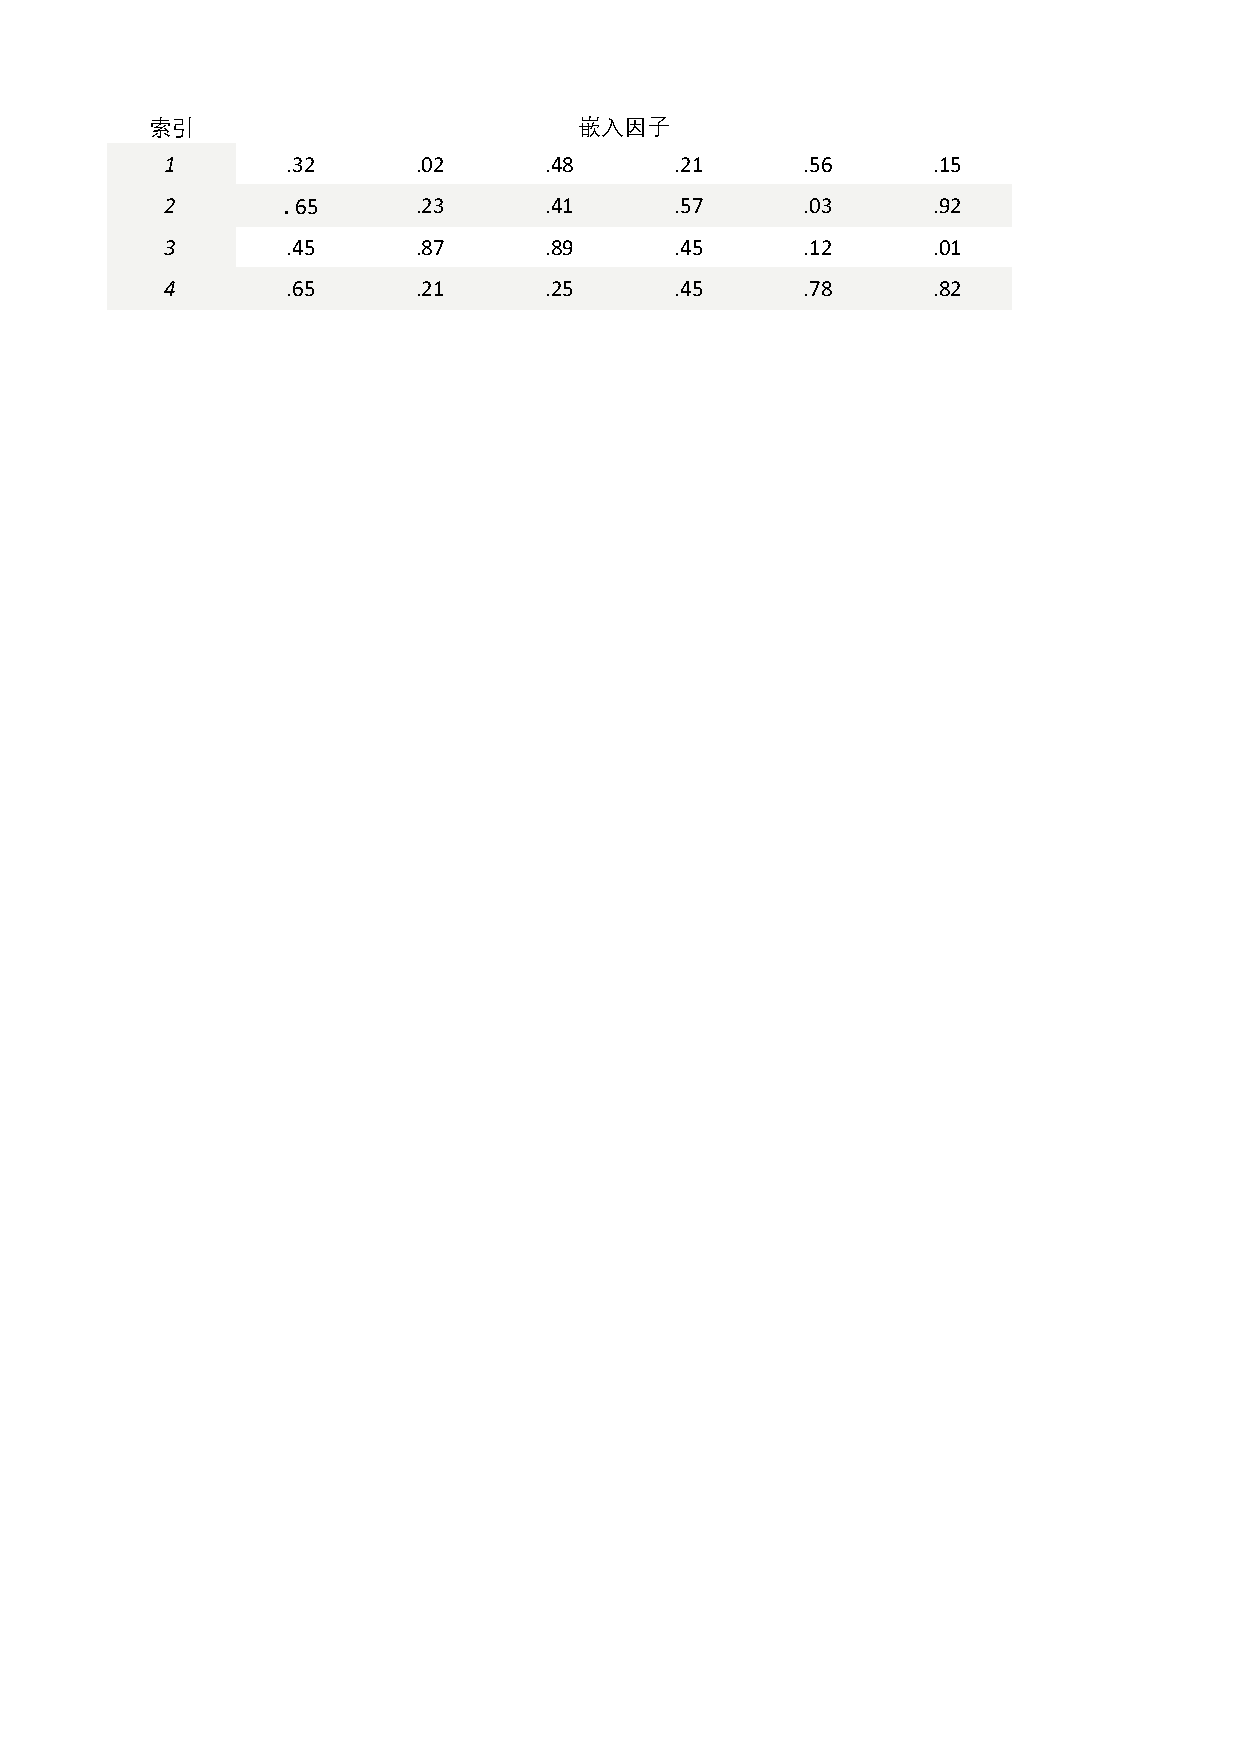
\includegraphics[width=\linewidth]{embedding.pdf}\\
  \caption{序列嵌入编码示意图}
  \label{fig:embedding}
\end{figure}
Embedding嵌入编码中并不是每一个物品ID都会被一个向量来代替,而是被替换为用于查找嵌入矩阵中向量的%
索引。其次这种方法面对大数据时也可有效计算。由于在深度神经网络的训练过程中嵌入向量也会被更新,还%
可以探索在高维空间中哪些物品之间具有彼此相似性。
\subsection{用户短期兴趣学习}
我们通过结合用户$u$在$t$时刻消费的项目$I_{u}^{t}$和其先后的项目来表达用户在此时刻的兴趣。行为序列帮助我们更精确地揭示了用户的短期兴趣。在这个推荐系统中,我们使用了一个双向的长短期记忆神经网络构建的循环结构来捕捉用户短期的兴趣变化。

我们定义$h_{b}(I_{i})$ 为用户他在消费物品$I_i$之前的兴趣,$h_{a}(I_{i})$为用户消费物品$I_i$之后的兴趣。$h_{b}(I_{i})$和$h_{a}(I_{i})$都是具有$|h|$个实数的稠密向量。$W^{(b)}$是隐藏层的权重矩阵,用来继承用户之前的兴趣状态,矩阵$W^{(cb)}$用来结合前一个物品的嵌入表达,$\sigma$是一个非线性激活函数,因此通过学习表达式$h_{b}(I_{i})$来学习用户消费物品$I_i$之前的兴趣。同理,用户消费物品$I_i$之后的兴趣通过学习表达式$h_{a}(I_{i})$来学习
。所有用户的初始兴趣使用同样的参数$h_{b}(I_{1})$,用户消费历史中的最后的兴趣则共享参数$h_{a}(I_{n})$。
\begin{align}
h_{b}(I_{i})=\sigma (W^{(b)}h_{b}(I_{i-1})+W^{(cb)}e(I_{i-1})) \\
h_{a}(I_{i})=\sigma (W^{(a)}h_{a}(I_{i+1})+W^{(ca)}e(I_{i+1}))
\end{align}
通过以上公式,学习用户某个时刻之前和之后的兴趣,将它们和用户当前消费物品的嵌入矩阵集合来表达此时刻用户的临时兴趣状态,其结合形式如下:
\begin{align}
x_{i}=[h_{b}(I_{i});e(I_{i});h_{a}(I_{i})]
\end{align}
所以通过使用大量用户的历史行为序列$\left \{ i_{1},i_{2},...,i_{n-1},i_{n} \right \}$,如果我们的模型学习到了某个用户消费物品$i_{n-1}$时的临时兴趣$x_{n-1}$,他将更有可能得到一个物品推荐$i_{n}$.双向循环结构能够对序列的前向扫描中捕获所有的$h_b$,反向扫描则捕获了所有的$h_a$。当训练集中所有的临时兴趣状态$x_i$都被捕获之后,运用一个线性转换与tanh激活函数将结果送到下一层。
\begin{align}
y_{i}^{(2)}=tanh(W^{(2)}x_{i}+b^{(2)})
\end{align}
$y_{i}^{(2)}$是潜在的兴趣向量,其中的每一个兴趣向量将通过上面权重和参数的更新来决定影响用户消费序列中最重要的因素。
\subsection{流行趋势学习}
群体的趋同性在推荐系统当中会产生一些热门点击物品,当某些信息较少的冷启动用户需要推荐时,尽管可能无法产生合理的个性化准确推荐结果,但直接为其推荐热门物品也不失为一个合理策略。
当用户消费项目的所有序列被计算完之后,接下来应用一个最大池化层:
\begin{align}
y^{(3)}=\max_{i=1}^{n}y_{i}^{(2)}
\end{align}
最大池化通过应用一个最大过滤器到上层代表的非重叠子区域,有了池化层,模型的参数或权重迅速减小了,这样也能减小上层输入的空间维度,减小计算消耗。通过对全局序列属性的捕获最大输出层能在用户的这个历史记录里找到那些最流行的序列组合。模型的最后一层就是常规的输出层了:
\begin{align}
y^{(4)}=W^{(4)}y^{(3)}+b^{(4)}
\end{align}
输出层通过应用一个softmax激活函数到$y^{(4)}$来转换成下一个类别的输出概率:
\begin{align}
p_{i}= \frac{e^{y_{i}^{(4)}}}{\sum_{k=1}^{n}e^{y_{k}^{(4)}}}
\end{align}
\subsection{模型的训练}
将模型训练过程中所有需要更新的参数定义为$\theta $。
\begin{equation}
\theta=  \left \{ E,b^{(2)},b^{(4)},h_{b}(B_{1}),h_{a}(B_{n}),W^{(2)}, W^{(4)},\right.\\
\left.W^{(b)},W^{(a)},W^{(b)},W^{(cb)},W^{(ca)} \right \} \\
\end{equation}
模型训练的优化目标是最小化交叉熵损失函数:
\begin{equation}
\mathcal{L}(y,S,\theta )=-\sum_{u\in \mathbb{U}}[y_{u}\log p(y_{u}|S_{u},\theta)+(1-y_{u})\log (1-p(y_{u}|S_{u},\theta ))]
\end{equation}
\section{复杂度分析}
在嵌入层当中,主要包含一个矩阵的向量乘积操作,这一部分的时间复杂度是$O(n)$。在双向长短期记忆网络中,网络的主体是LSTM,其时间复杂度为$O(n\cdot d^{2})$,$n$表示序列的长度,$d$表示嵌入层因子的维度。而双向LSTM的时间复杂度我们可以知道为$2\cdot O(n\cdot d^{2})$,最大池化层的时间复杂度为$O(n)$,全连接层的时间复杂度为$O(n)$,整个模型是上述这些结构的串联,所以整个基于双向循环神经网络的序列推荐算法的时间复杂度为$O(n\cdot d^{2})$。相比于基于用户的协同过滤算法(UBCF)\upcite{Resnick:1994:GOA:192844.192905}的时间复杂度$O(n_{u}^{2})$和基于物品的协同过滤(IBCF)\upcite{Sarwar:2001:ICF:371920.372071}时间复杂度$O(n_{i}^{2})$,其中$n_{u}$表示用户数量,$n_{i}$表示物品数量。与其相比,序列长度$n$和嵌入维度$d$存在这样的关系:$n_{u}> n_{i}\gg d> n$,所以基于双向循环神经网络的序列推荐算法在选择合适的序列长度和嵌入维度大小时面对大数据处理的压力时还是可以接受的。
\section{算法实现}
\begin{algorithm}[htbp]
	\caption{基于双向长短期记忆网络的序列感知推荐算法}
	\label{alg:bi-lstm}
		\begin{algorithmic}[1]
			\REQUIRE 用户序列数据:$S$;序列长度:$maxLen$; 最大物品数:$maxNum$
			\ENSURE 推荐结果:$Items$
			\STATE $sequence \leftarrow S$, 其中$sequence=\{seq_{1}, seq_{2}...seq_{n}\}$
			\IF {$len(sequence) >= maxLen$}
				\STATE 选取序列最后的N物品:$sentences_{lastn} \subseteqq sequence$
			  	\STATE $items \leftarrow sequence_{topn}$,其中 $items=\{word_{1}, word_{2}...word_{m}\}$
			  \FOR{each $i \in [1,maxLen]$}
			    \STATE 将每个序列的物品ID编码到嵌入矩阵:$E = Embedding_{seq_{i}}$
			  \ENDFOR
			  
			\ELSE
				\STATE continue
			\ENDIF
			\FOR{each $i \in [1, maxLen]$}
				\STATE $output_{right}$ = LSTM(E)
				\ENDFOR
			\FOR{each $i \in [maxLen, 1]$}
				\STATE $output_{left}$ = LSTM(E)
				\ENDFOR
			\STATE $output$ = $[output_{right}; output_{left}]$
			\STATE $output$ = $maxpolling(output)$
			\STATE $NextItem = SoftMax(output) $
			\RETURN $NextItem$
		\end{algorithmic}
\end{algorithm}
BiLSTM4Rec算法的主要流程如伪代码\ref{alg:bi-lstm}所示,处理成序列形式的特征数据输入给模型训练,其序列长度应截取为$maxLen$大小,而模型则由嵌入层、双向LSTM循环层、池化层、全连接输出层依次堆叠而成。最后将输出概率最高的$N$个物品返回作为推荐序列。
\section{本章小结}

本章节主要介绍本文提出的一个针对用户下一个点击推荐的新颖神经网络推荐模型BiLSTM4Rec,其利用双向长短期记忆网络来对用户按照时间先后点击物品的历史记录进行序列建模,挖掘隐藏在序列当中的用户短期兴趣变化,来精确地对用户下一个可能感兴趣的物品做出推荐。通过对大规模物品ID进行矩阵嵌入压缩处理,借助该时序推荐算法,能够取得比传统协同过滤更高效更精确地短期推荐策略。

